\documentclass[isoft]{ufgtexposter}

\usepackage{lipsum}
\usepackage{natbib}
\usepackage{booktabs}
\usepackage{subfig} 
\usepackage{amsmath} 
\usepackage{textcomp} 
\usepackage{url}  
\usepackage[hidelinks]{hyperref}
\usepackage[utf8]{inputenc}
\usepackage[spanish]{babel}

%%%%%%%%%%%%%%%%%%%%%%%%%%%%%%%%%%%%%%%%%
%%               Configs               %%
%%%%%%%%%%%%%%%%%%%%%%%%%%%%%%%%%%%%%%%%%

% Choose one of the section color {ufglhblue | ufgdkblue | dkblue | black | gold}
\setsectioncolor{ufgdkblue} 

% Define width of the rule or hide it by setting 0pt or commenting the command 
\setcolumnseprule{0pt}

% Inform the paths to the logo files or leave empty one or both parameters. 
% There are three options [ T | M | B ] to positioning them.
%logo de episi y unam
\setlogos[M]{images/episi}{images/unamc}

% Choose one of the background options {1 | 2 | 3}. 
% Actually, one can select any graphic file in backgrounds directory. 
\setbackground{1.pdf}

% Resize the title to keep it in two lines // {font size}{line height}
\settitlesize{64pt}{68pt}

% Resize the font of the content. Default {32pt}{38pt} // {font size}{line height}
\setcontentfontesize{32pt}{40pt}

% Resize the font of the emails. Default {26pt}{32pt} // {font size}{line height}
\setemailfontesize{42pt}{40pt}

% General info
\title{\uppercase{Titulo oficial de su \\ proyecto de innovación}} 
\author{Nombre Apellidos, Nombre Apellidos, Nombre Apellidos} 

\department{Ingeniería de Sistemas e Informática, UNAM, Perú}

\email{ \text{email@gmail.com, email@gmail.com, email@gmail.com} }

\class{I Feria de Proyectos EPISI 2022-I}

\posteryear{2022}

\copyrightholder{I Feria de Proyectos EPISI 2022-I, UNAM, Ilo, Perú }

%%%%%%%%%%%%%%%%%%%%%%%%%%%%%%%%%%%%%%%%%
%%           End configs               %%
%%%%%%%%%%%%%%%%%%%%%%%%%%%%%%%%%%%%%%%%%

\pagestyle{fancy}
\begin{document}
    \begin{poster}
    %%%%%%%%%%%%%%%%%%%%%%%%%%%%%%%%%%%%%%%%%
    %%             Begin poster            %%
    %%%%%%%%%%%%%%%%%%%%%%%%%%%%%%%%%%%%%%%%%
    
    \section{Resumen}
    Following the report of Internet World Stats 2019 \cite{b1}, the access to the Internet and web technology has grown fastly and let the users interact trough different platforms. Considering the demand and offer of job, exist a lot of data with no structure, the websites related to job offer usually has the Curriculum Vitae about the candidates and job offers.
    Recommendation Systems are useful to suggest or recommend one item to one user based on the information from other users or content similar. Frequently the users have specific preferences \cite{b2} for some products, the preferences are present in non-explicit text and explicit data.
    This research project on line Text Mining \cite{b3} and Natural Language Processing(NLP)is about how to represent and use the information from the text written by human beings on web sites for job offer recommendation.
        
    \section{Objetivos}%
    \begin{figure}
            \centering
            \captionsetup{type=figure}
            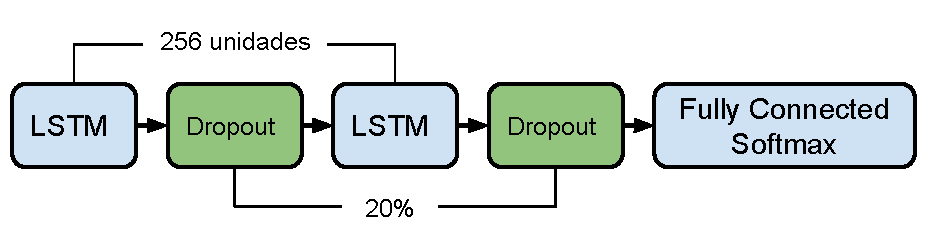
\includegraphics[scale=2.3]{modelo-lstm}
            \caption{Arquitetura da rede LSTM utilizada no trabalho.}
            \label{fig:lstm}
    \end{figure}
    \section{Metodología}
    
        
        \subsection{Information  retrieval}
        
        \lipsum[11]
        
        \vspace{1cm}
        
        
        
        \subsection{Coloque aqui seu \textit{dataset}}
        
            \lipsum[54]
            
            \vspace{1cm}
            \begin{table}
                \centering
                \captionsetup{type=table}
                \caption{\textit{Corpus} utilizados no estudo}
                \label{Corpus}
                \renewcommand{\arraystretch}{1.2}
                \resizebox{0.47\textwidth}{!}{%
                \begin{tabular}{lcccclcl}
                    \hline
                    &\textbf{Corpus}    &  \textbf{Caracteres únicos} &    &  \textbf{Total de linhas}  &  & \textbf{Total de caracteres} &  \\ \hline
                    &SBSEThesis         & 88  &    &    2.311     &        & 771.179 &  \\ 
                    &Bible              & 63  &    &    32.359   &        & 3.924.374 &  \\
                    &JavaCode           & 69  &    &    436.565  &        & 12.053.424 &  \\ \hline
                \end{tabular}
            }
            \end{table}
            \vspace{1cm}
            
            \lipsum[57]
            
            \citep{b1}.
    
            \subsection{Subsection}
                \lipsum[8]
    
        \section{Resultados}%
                
            On the results of the previous stage, we can analyze and visualize the usefulness of this data, the results can help different cases. In the Figure 1, we can see a matrix of 5000 resumes for 9998 jobs (5000x9998), where the relevance value of each curriculum vitae is distributed on a matrix basis.    
            
    
            \begin{figure}
                \centering
                \captionsetup{type=figure}
                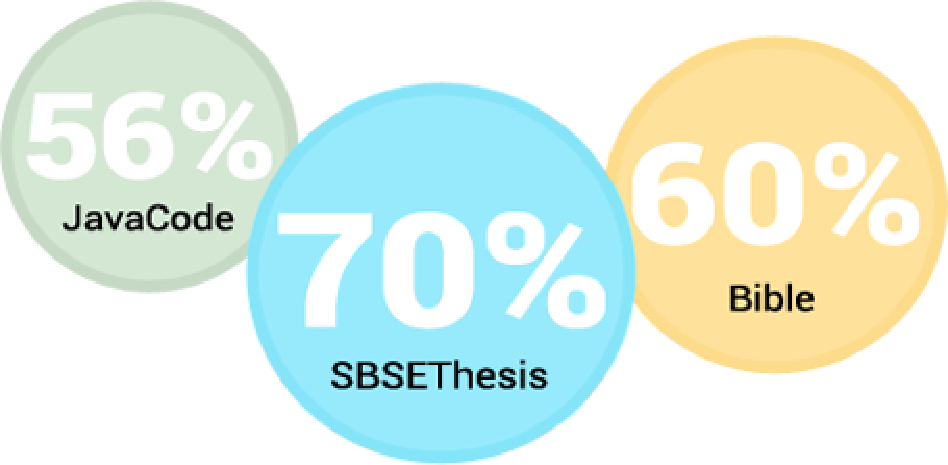
\includegraphics[scale=2]{resultado}
                \caption{Taxa de sucesso de predição por \textit{corpus}.}
                \label{fig:result}
            \end{figure}
    
            \lipsum[5]
            \cite{b2}     
    

    
            \lipsum[15]
    
        \section{Conclusiones}
    
            \lipsum[57]
        \bibliographystyle{plain} % We choose the "plain" reference style
        \bibliography{refs}
    
    %%%%%%%%%%%%%%%%%%%%%%%%%%%%%%%%%%%%%%%%%
    %%               End poster            %%
    %%%%%%%%%%%%%%%%%%%%%%%%%%%%%%%%%%%%%%%%%
    
    \end{poster}

\end{document}

 
